\subsection{Chap 1 } \label{chap1}

\subsubsection*{Question 1}

\begin{equation}
    \sigma = \frac{N e^2 \tau}{m^*}
\end{equation}


At it is a monovalent metal and the FCC-Unit cell contains 
4 atoms the concentration of the conduction electrons $N$ can be
calculated as:
$$N =\frac{4}{a^3}$$

So for the collision time $\tau$ follows:
With $(m^* = m_0)$ the free electron mass.

The electrical resitivity is given as:
$\rho = 2.13 \mu \Omega cm$

which leads to a conducitivity of
$\sigma = \frac{1}{\rho} = 4.695\cdot 10^7 \frac{1}{\Omega m}$

$a = 4.09 \mathring{A}$

$$\tau =\frac{\sigma \cdot m^* \cdot a^3}{4e^2} = 28.5 \cdot 10^{-14}s$$

\subsubsection*{Question 2}

For a thin metal wire with a length of $10 \, cm$, a square cross section with 
a side of $0.1 \, mm$ and a potential difference along the wire of $0.2 \, V$

The electric field $E$ in the wire can be calculated as: 

$$E = \frac{U}{L} = 2 \frac{V}{m}$$

As for the current density the following relations are known.

$$J = \sigma E \qquad J = nev_D$$

So for the drift velocitiy follows:

$$v_D =  \frac{\sigma E}{n e}$$

\subsubsection*{Question 3}


\subsubsection*{Fermi}

The energy of the electron in a metal is quantized according to quantum mechanics.
As so they follow the \textit{Pauli exclusiion principle}, which means only two 
electrons with diffenrent spin can occupy one energy level.
The highest occupied energy level is then called the Fermi energy or the fermy
level.

The situation described obtains in metals as $T=0 \degree K$. The probability that 
an level below the fermi energy is occupied is 1 and above equals 0.

If the system is heated, the electrons near the fermi level get excited as 
the electrons below the fermi level can not absorb energy due to the exclusiion
principle.

Which leads to the \textit{Fermi-Dirac distribution}, which gives
the probability that the level $E$ is occupied by an electron.

\begin{equation}
    f(E) = \frac{1}{e^{(E-E_F)/kT}+1}
\end{equation}

\begin{figure}[H]
    \centering
    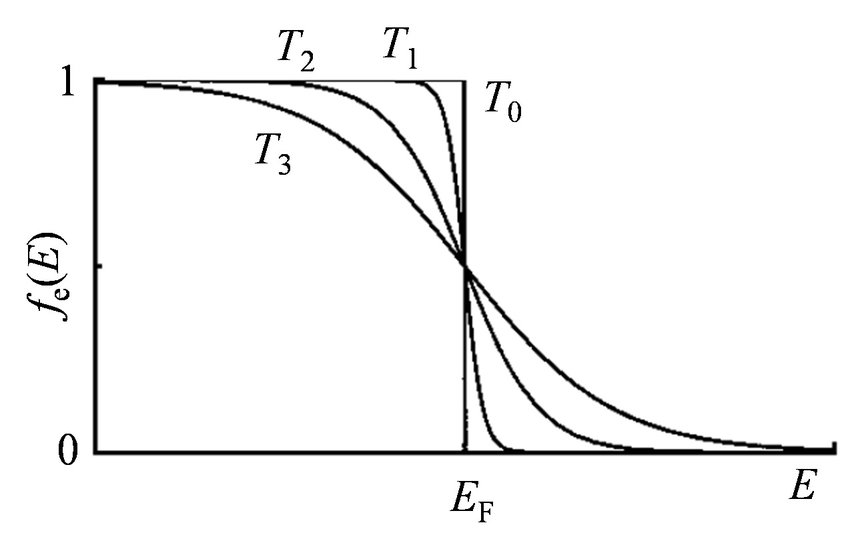
\includegraphics[width=0.5\linewidth]{Graphics/Chapter1/Fermi-Dirac-distribution.png}
    \caption{Fermi-Dirac distribution function at different temperatures: T3> T2>T1
     (and T0 = 0 K). At the absolute zero temperature (T0), the probability of an 
     electron to have an energy below the Fermi energy EF is equal to 1, while the 
     probability to have higher energy is zero.}
    \label{}
\end{figure}

As the energy of an electron is entirely kinetic, it is possible
to write the energy as:

$$E = \frac{1}{2} m^* v^2$$

As for the $T=0 \degree$ the fermi energy is the highest possible value
a maximum velocitiy $v_F$ of the particles can be found. 

$$E_F = m^*v_F^2$$

This leads to a shere in the three dimesional velocitiy space
$(v_x, \, v_y, \, v_z)$ the sphere has an radius of $v_F$


\begin{figure}[H]
    \centering
    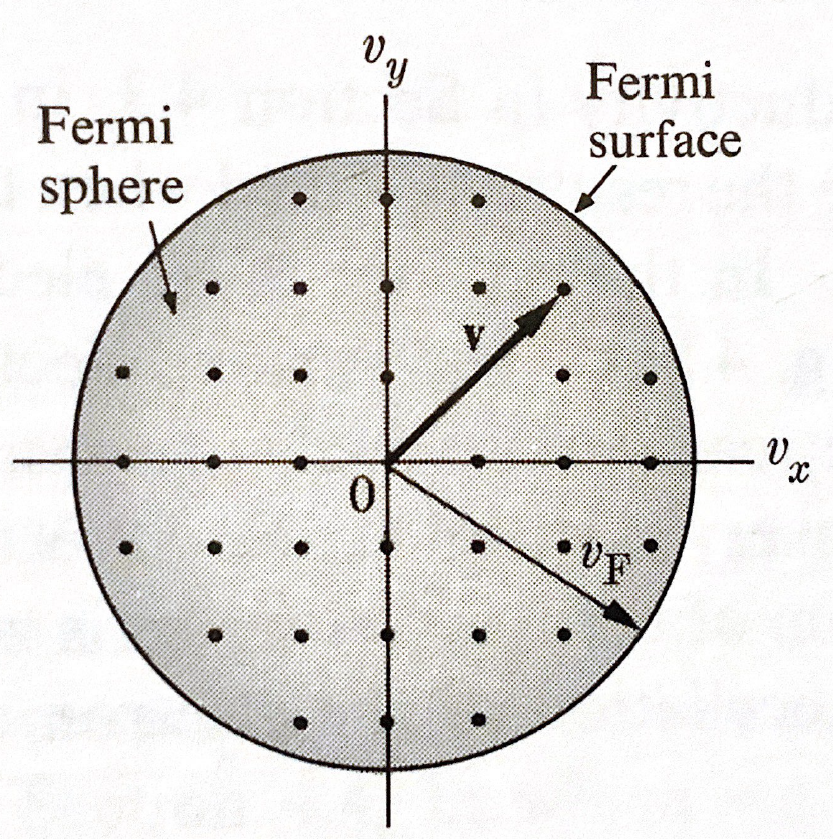
\includegraphics[width=0.4\linewidth]{Graphics/Chapter1/Fermi_Sphere.png}
    \caption{The Fermi surface and the Fermi sphere \cite[asdfadf]{elementary_SSP} }
    \label{}
\end{figure}

\subsubsection*{Cyclotron}
\begin{equation}
    -e (\vec{v} \times \vec{B}) =  m \frac{d\vec{v}}{dt}
\end{equation}

With the given information that $\vec{B} = B\vec{z}$
The equation above lead to the following:

$-e v_y B = m \frac{d}{dt}v_x$\\
$e v_x B = m \frac{d}{dt}v_y$

Which can be solved with the additional information

$$x = k_{0x}$$

$$\omega = \frac{eB}{m^*}$$

\subsubsection*{Plasma Frequency}

\begin{equation}
    w_P = \frac{Ne^2}{\epsilon_L m^*}
\end{equation}

With the parameter given

$m^*=m_0$

$\epsilon_L = \epsilon_0$

Tha plasma frequency can be calculated as:

$$w_P = 1.861 \cdot 10^{11} \frac{1}{s}$$